% Options for packages loaded elsewhere
\PassOptionsToPackage{unicode}{hyperref}
\PassOptionsToPackage{hyphens}{url}
\PassOptionsToPackage{dvipsnames,svgnames,x11names}{xcolor}
%
\documentclass[
  letterpaper,
  DIV=11,
  numbers=noendperiod]{scrartcl}

\usepackage{amsmath,amssymb}
\usepackage{iftex}
\ifPDFTeX
  \usepackage[T1]{fontenc}
  \usepackage[utf8]{inputenc}
  \usepackage{textcomp} % provide euro and other symbols
\else % if luatex or xetex
  \usepackage{unicode-math}
  \defaultfontfeatures{Scale=MatchLowercase}
  \defaultfontfeatures[\rmfamily]{Ligatures=TeX,Scale=1}
\fi
\usepackage{lmodern}
\ifPDFTeX\else  
    % xetex/luatex font selection
\fi
% Use upquote if available, for straight quotes in verbatim environments
\IfFileExists{upquote.sty}{\usepackage{upquote}}{}
\IfFileExists{microtype.sty}{% use microtype if available
  \usepackage[]{microtype}
  \UseMicrotypeSet[protrusion]{basicmath} % disable protrusion for tt fonts
}{}
\makeatletter
\@ifundefined{KOMAClassName}{% if non-KOMA class
  \IfFileExists{parskip.sty}{%
    \usepackage{parskip}
  }{% else
    \setlength{\parindent}{0pt}
    \setlength{\parskip}{6pt plus 2pt minus 1pt}}
}{% if KOMA class
  \KOMAoptions{parskip=half}}
\makeatother
\usepackage{xcolor}
\setlength{\emergencystretch}{3em} % prevent overfull lines
\setcounter{secnumdepth}{-\maxdimen} % remove section numbering
% Make \paragraph and \subparagraph free-standing
\ifx\paragraph\undefined\else
  \let\oldparagraph\paragraph
  \renewcommand{\paragraph}[1]{\oldparagraph{#1}\mbox{}}
\fi
\ifx\subparagraph\undefined\else
  \let\oldsubparagraph\subparagraph
  \renewcommand{\subparagraph}[1]{\oldsubparagraph{#1}\mbox{}}
\fi

\usepackage{color}
\usepackage{fancyvrb}
\newcommand{\VerbBar}{|}
\newcommand{\VERB}{\Verb[commandchars=\\\{\}]}
\DefineVerbatimEnvironment{Highlighting}{Verbatim}{commandchars=\\\{\}}
% Add ',fontsize=\small' for more characters per line
\usepackage{framed}
\definecolor{shadecolor}{RGB}{241,243,245}
\newenvironment{Shaded}{\begin{snugshade}}{\end{snugshade}}
\newcommand{\AlertTok}[1]{\textcolor[rgb]{0.68,0.00,0.00}{#1}}
\newcommand{\AnnotationTok}[1]{\textcolor[rgb]{0.37,0.37,0.37}{#1}}
\newcommand{\AttributeTok}[1]{\textcolor[rgb]{0.40,0.45,0.13}{#1}}
\newcommand{\BaseNTok}[1]{\textcolor[rgb]{0.68,0.00,0.00}{#1}}
\newcommand{\BuiltInTok}[1]{\textcolor[rgb]{0.00,0.23,0.31}{#1}}
\newcommand{\CharTok}[1]{\textcolor[rgb]{0.13,0.47,0.30}{#1}}
\newcommand{\CommentTok}[1]{\textcolor[rgb]{0.37,0.37,0.37}{#1}}
\newcommand{\CommentVarTok}[1]{\textcolor[rgb]{0.37,0.37,0.37}{\textit{#1}}}
\newcommand{\ConstantTok}[1]{\textcolor[rgb]{0.56,0.35,0.01}{#1}}
\newcommand{\ControlFlowTok}[1]{\textcolor[rgb]{0.00,0.23,0.31}{#1}}
\newcommand{\DataTypeTok}[1]{\textcolor[rgb]{0.68,0.00,0.00}{#1}}
\newcommand{\DecValTok}[1]{\textcolor[rgb]{0.68,0.00,0.00}{#1}}
\newcommand{\DocumentationTok}[1]{\textcolor[rgb]{0.37,0.37,0.37}{\textit{#1}}}
\newcommand{\ErrorTok}[1]{\textcolor[rgb]{0.68,0.00,0.00}{#1}}
\newcommand{\ExtensionTok}[1]{\textcolor[rgb]{0.00,0.23,0.31}{#1}}
\newcommand{\FloatTok}[1]{\textcolor[rgb]{0.68,0.00,0.00}{#1}}
\newcommand{\FunctionTok}[1]{\textcolor[rgb]{0.28,0.35,0.67}{#1}}
\newcommand{\ImportTok}[1]{\textcolor[rgb]{0.00,0.46,0.62}{#1}}
\newcommand{\InformationTok}[1]{\textcolor[rgb]{0.37,0.37,0.37}{#1}}
\newcommand{\KeywordTok}[1]{\textcolor[rgb]{0.00,0.23,0.31}{#1}}
\newcommand{\NormalTok}[1]{\textcolor[rgb]{0.00,0.23,0.31}{#1}}
\newcommand{\OperatorTok}[1]{\textcolor[rgb]{0.37,0.37,0.37}{#1}}
\newcommand{\OtherTok}[1]{\textcolor[rgb]{0.00,0.23,0.31}{#1}}
\newcommand{\PreprocessorTok}[1]{\textcolor[rgb]{0.68,0.00,0.00}{#1}}
\newcommand{\RegionMarkerTok}[1]{\textcolor[rgb]{0.00,0.23,0.31}{#1}}
\newcommand{\SpecialCharTok}[1]{\textcolor[rgb]{0.37,0.37,0.37}{#1}}
\newcommand{\SpecialStringTok}[1]{\textcolor[rgb]{0.13,0.47,0.30}{#1}}
\newcommand{\StringTok}[1]{\textcolor[rgb]{0.13,0.47,0.30}{#1}}
\newcommand{\VariableTok}[1]{\textcolor[rgb]{0.07,0.07,0.07}{#1}}
\newcommand{\VerbatimStringTok}[1]{\textcolor[rgb]{0.13,0.47,0.30}{#1}}
\newcommand{\WarningTok}[1]{\textcolor[rgb]{0.37,0.37,0.37}{\textit{#1}}}

\providecommand{\tightlist}{%
  \setlength{\itemsep}{0pt}\setlength{\parskip}{0pt}}\usepackage{longtable,booktabs,array}
\usepackage{calc} % for calculating minipage widths
% Correct order of tables after \paragraph or \subparagraph
\usepackage{etoolbox}
\makeatletter
\patchcmd\longtable{\par}{\if@noskipsec\mbox{}\fi\par}{}{}
\makeatother
% Allow footnotes in longtable head/foot
\IfFileExists{footnotehyper.sty}{\usepackage{footnotehyper}}{\usepackage{footnote}}
\makesavenoteenv{longtable}
\usepackage{graphicx}
\makeatletter
\def\maxwidth{\ifdim\Gin@nat@width>\linewidth\linewidth\else\Gin@nat@width\fi}
\def\maxheight{\ifdim\Gin@nat@height>\textheight\textheight\else\Gin@nat@height\fi}
\makeatother
% Scale images if necessary, so that they will not overflow the page
% margins by default, and it is still possible to overwrite the defaults
% using explicit options in \includegraphics[width, height, ...]{}
\setkeys{Gin}{width=\maxwidth,height=\maxheight,keepaspectratio}
% Set default figure placement to htbp
\makeatletter
\def\fps@figure{htbp}
\makeatother

\KOMAoption{captions}{tableheading}
\makeatletter
\@ifpackageloaded{caption}{}{\usepackage{caption}}
\AtBeginDocument{%
\ifdefined\contentsname
  \renewcommand*\contentsname{Table of contents}
\else
  \newcommand\contentsname{Table of contents}
\fi
\ifdefined\listfigurename
  \renewcommand*\listfigurename{List of Figures}
\else
  \newcommand\listfigurename{List of Figures}
\fi
\ifdefined\listtablename
  \renewcommand*\listtablename{List of Tables}
\else
  \newcommand\listtablename{List of Tables}
\fi
\ifdefined\figurename
  \renewcommand*\figurename{Figure}
\else
  \newcommand\figurename{Figure}
\fi
\ifdefined\tablename
  \renewcommand*\tablename{Table}
\else
  \newcommand\tablename{Table}
\fi
}
\@ifpackageloaded{float}{}{\usepackage{float}}
\floatstyle{ruled}
\@ifundefined{c@chapter}{\newfloat{codelisting}{h}{lop}}{\newfloat{codelisting}{h}{lop}[chapter]}
\floatname{codelisting}{Listing}
\newcommand*\listoflistings{\listof{codelisting}{List of Listings}}
\makeatother
\makeatletter
\makeatother
\makeatletter
\@ifpackageloaded{caption}{}{\usepackage{caption}}
\@ifpackageloaded{subcaption}{}{\usepackage{subcaption}}
\makeatother
\ifLuaTeX
  \usepackage{selnolig}  % disable illegal ligatures
\fi
\usepackage{bookmark}

\IfFileExists{xurl.sty}{\usepackage{xurl}}{} % add URL line breaks if available
\urlstyle{same} % disable monospaced font for URLs
\hypersetup{
  pdftitle={DATA 605 Assignment 1},
  pdfauthor={Amanda Fox},
  colorlinks=true,
  linkcolor={blue},
  filecolor={Maroon},
  citecolor={Blue},
  urlcolor={Blue},
  pdfcreator={LaTeX via pandoc}}

\title{DATA 605 Assignment 1}
\author{Amanda Fox}
\date{}

\begin{document}
\maketitle

Load libraries:

\begin{Shaded}
\begin{Highlighting}[]
\CommentTok{\# load libraries}
\FunctionTok{library}\NormalTok{(tidyverse)}
\FunctionTok{library}\NormalTok{(ggplot2)}
\FunctionTok{library}\NormalTok{(patchwork)}
\FunctionTok{library}\NormalTok{(jpeg)}
\FunctionTok{library}\NormalTok{(RCurl)}
\end{Highlighting}
\end{Shaded}

\subsubsection{1. Task: Create a simple shape (like a square or
triangle) using point plots in R. Implement R code to apply different
transformations (scaling, rotation, reflection) to the shape by left
multiplying a transformation matrix by each of the point vectors.
Demonstrate these transformations through animated
plots.}\label{task-create-a-simple-shape-like-a-square-or-triangle-using-point-plots-in-r.-implement-r-code-to-apply-different-transformations-scaling-rotation-reflection-to-the-shape-by-left-multiplying-a-transformation-matrix-by-each-of-the-point-vectors.-demonstrate-these-transformations-through-animated-plots.}

To create a triangle, we use a 2x4 matrix: the first three columns
represent three point vectors (x,y) and the fourth column repeats the
first point vector to close the shape.

\begin{Shaded}
\begin{Highlighting}[]
\CommentTok{\# create matrix defining triangle:}
\NormalTok{my\_shape }\OtherTok{\textless{}{-}} \FunctionTok{matrix}\NormalTok{(}\FunctionTok{c}\NormalTok{(}\DecValTok{0}\NormalTok{,}\DecValTok{0}\NormalTok{,}
                     \DecValTok{1}\NormalTok{,}\DecValTok{0}\NormalTok{,}
                     \DecValTok{0}\NormalTok{,}\DecValTok{1}\NormalTok{,}
                     \DecValTok{0}\NormalTok{,}\DecValTok{0}\NormalTok{), }
                   \AttributeTok{nrow =} \DecValTok{2}\NormalTok{, }\AttributeTok{byrow =} \ConstantTok{TRUE}\NormalTok{)}
\NormalTok{my\_shape}
\end{Highlighting}
\end{Shaded}

\begin{verbatim}
     [,1] [,2] [,3] [,4]
[1,]    0    0    1    0
[2,]    0    1    0    0
\end{verbatim}

\begin{Shaded}
\begin{Highlighting}[]
\CommentTok{\# prepare to plot: convert to df and label columns x \& y}
\NormalTok{df\_my\_shape }\OtherTok{\textless{}{-}} \FunctionTok{as.data.frame}\NormalTok{(}\FunctionTok{t}\NormalTok{(my\_shape))  }
\FunctionTok{colnames}\NormalTok{(df\_my\_shape) }\OtherTok{\textless{}{-}} \FunctionTok{c}\NormalTok{(}\StringTok{"x"}\NormalTok{,}\StringTok{"y"}\NormalTok{)}

\NormalTok{df\_my\_shape}
\end{Highlighting}
\end{Shaded}

\begin{verbatim}
  x y
1 0 0
2 0 1
3 1 0
4 0 0
\end{verbatim}

\begin{Shaded}
\begin{Highlighting}[]
\CommentTok{\# plot}
\NormalTok{plot\_my\_shape }\OtherTok{\textless{}{-}}\NormalTok{ df\_my\_shape }\SpecialCharTok{\%\textgreater{}\%} 
  \FunctionTok{ggplot}\NormalTok{(}\FunctionTok{aes}\NormalTok{(}\AttributeTok{x =}\NormalTok{ x, }\AttributeTok{y =}\NormalTok{ y)) }\SpecialCharTok{+}
         \FunctionTok{geom\_path}\NormalTok{(}\AttributeTok{color =} \StringTok{\textquotesingle{}blue\textquotesingle{}}\NormalTok{, }\AttributeTok{linewidth =} \FloatTok{1.2}\NormalTok{) }\SpecialCharTok{+}
         \FunctionTok{geom\_hline}\NormalTok{(}\AttributeTok{yintercept =} \DecValTok{0}\NormalTok{, }\AttributeTok{color =} \StringTok{"gray30"}\NormalTok{) }\SpecialCharTok{+}
         \FunctionTok{geom\_vline}\NormalTok{(}\AttributeTok{xintercept =} \DecValTok{0}\NormalTok{, }\AttributeTok{color =} \StringTok{"gray30"}\NormalTok{) }\SpecialCharTok{+}
         \FunctionTok{coord\_fixed}\NormalTok{(}\AttributeTok{xlim =} \FunctionTok{c}\NormalTok{(}\SpecialCharTok{{-}}\DecValTok{2}\NormalTok{,}\DecValTok{2}\NormalTok{), }\AttributeTok{ylim =} \FunctionTok{c}\NormalTok{(}\SpecialCharTok{{-}}\DecValTok{2}\NormalTok{,}\DecValTok{2}\NormalTok{)) }\SpecialCharTok{+}
         \FunctionTok{theme\_minimal}\NormalTok{()}

\NormalTok{plot\_my\_shape }\SpecialCharTok{+} \FunctionTok{plot\_annotation}\NormalTok{(}\StringTok{"Original Triangle"}\NormalTok{)}
\end{Highlighting}
\end{Shaded}

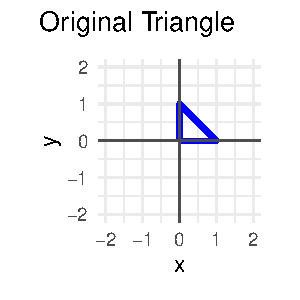
\includegraphics{Assignment-1---Fox_files/figure-pdf/create_shape-1.pdf}

Next, we can scale the shape by multiplying it by a transformation
matrix. In this case, we set up our transformation matrix to multiply
both x and y by 2:

\begin{Shaded}
\begin{Highlighting}[]
\CommentTok{\# create scaling transformation matrix multiplying x and y by 2 }
\NormalTok{matrix\_scale }\OtherTok{\textless{}{-}} \FunctionTok{matrix}\NormalTok{(}\FunctionTok{c}\NormalTok{(}\DecValTok{2}\NormalTok{,}\DecValTok{0}\NormalTok{,}
                         \DecValTok{0}\NormalTok{,}\DecValTok{2}\NormalTok{),}
                       \AttributeTok{nrow =} \DecValTok{2}\NormalTok{, }\AttributeTok{byrow =} \ConstantTok{TRUE}\NormalTok{)}
\NormalTok{matrix\_scale}
\end{Highlighting}
\end{Shaded}

\begin{verbatim}
     [,1] [,2]
[1,]    2    0
[2,]    0    2
\end{verbatim}

\begin{Shaded}
\begin{Highlighting}[]
\CommentTok{\# multiply: transpose my\_shape matrix so \# rows match \# columns }
\NormalTok{my\_shape\_scaled }\OtherTok{\textless{}{-}} \FunctionTok{t}\NormalTok{(my\_shape) }\SpecialCharTok{\%*\%}\NormalTok{ matrix\_scale }
\NormalTok{my\_shape\_scaled}
\end{Highlighting}
\end{Shaded}

\begin{verbatim}
     [,1] [,2]
[1,]    0    0
[2,]    0    2
[3,]    2    0
[4,]    0    0
\end{verbatim}

\begin{Shaded}
\begin{Highlighting}[]
\CommentTok{\# convert to df with column names x,y}
\NormalTok{df\_my\_shape\_scaled }\OtherTok{\textless{}{-}} \FunctionTok{as.data.frame}\NormalTok{(my\_shape\_scaled)  }
\FunctionTok{colnames}\NormalTok{(df\_my\_shape\_scaled) }\OtherTok{\textless{}{-}} \FunctionTok{c}\NormalTok{(}\StringTok{"x"}\NormalTok{,}\StringTok{"y"}\NormalTok{)}

\NormalTok{df\_my\_shape\_scaled}
\end{Highlighting}
\end{Shaded}

\begin{verbatim}
  x y
1 0 0
2 0 2
3 2 0
4 0 0
\end{verbatim}

\begin{Shaded}
\begin{Highlighting}[]
\CommentTok{\# plot}
\NormalTok{plot\_my\_shape\_scaled }\OtherTok{\textless{}{-}}\NormalTok{ df\_my\_shape\_scaled }\SpecialCharTok{\%\textgreater{}\%} 
  \FunctionTok{ggplot}\NormalTok{(}\FunctionTok{aes}\NormalTok{(}\AttributeTok{x =}\NormalTok{ x, }\AttributeTok{y =}\NormalTok{ y)) }\SpecialCharTok{+}
  \FunctionTok{geom\_path}\NormalTok{(}\AttributeTok{color =} \StringTok{\textquotesingle{}blue\textquotesingle{}}\NormalTok{, }\AttributeTok{linewidth =} \FloatTok{1.2}\NormalTok{) }\SpecialCharTok{+}
  \FunctionTok{geom\_hline}\NormalTok{(}\AttributeTok{yintercept =} \DecValTok{0}\NormalTok{, }\AttributeTok{color =} \StringTok{"gray30"}\NormalTok{) }\SpecialCharTok{+}
  \FunctionTok{geom\_vline}\NormalTok{(}\AttributeTok{xintercept =} \DecValTok{0}\NormalTok{, }\AttributeTok{color =} \StringTok{"gray30"}\NormalTok{) }\SpecialCharTok{+}
  \FunctionTok{coord\_fixed}\NormalTok{(}\AttributeTok{xlim =} \FunctionTok{c}\NormalTok{(}\SpecialCharTok{{-}}\DecValTok{2}\NormalTok{,}\DecValTok{2}\NormalTok{), }\AttributeTok{ylim =} \FunctionTok{c}\NormalTok{(}\SpecialCharTok{{-}}\DecValTok{2}\NormalTok{,}\DecValTok{2}\NormalTok{)) }\SpecialCharTok{+}
  \FunctionTok{theme\_minimal}\NormalTok{()}

\NormalTok{plot\_my\_shape }\SpecialCharTok{+}\NormalTok{ plot\_my\_shape\_scaled  }\SpecialCharTok{+} \FunctionTok{plot\_annotation}\NormalTok{(}\StringTok{"Original and Scaled Triangle"}\NormalTok{)}
\end{Highlighting}
\end{Shaded}

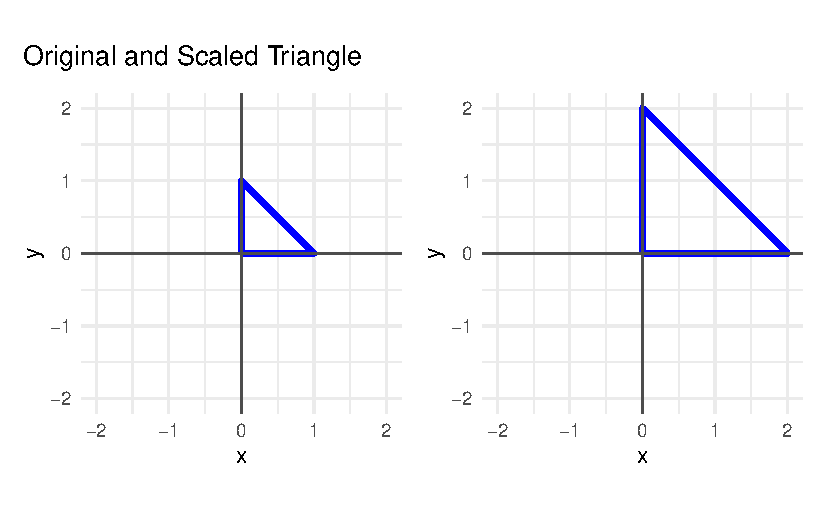
\includegraphics{Assignment-1---Fox_files/figure-pdf/scale-1.pdf}

We can also use a transformation matrix to flip our shape over. In the
example below, we create a transformation matrix to flip the shape over
the x axis by keeping x values the same while multiplying y values by
-1:

\begin{Shaded}
\begin{Highlighting}[]
\CommentTok{\# create transformation matrix (x, y) → (x, {-}y)}
\NormalTok{matrix\_flip }\OtherTok{\textless{}{-}} \FunctionTok{matrix}\NormalTok{(}\FunctionTok{c}\NormalTok{(}\DecValTok{1}\NormalTok{, }\DecValTok{0}\NormalTok{,}
                        \DecValTok{0}\NormalTok{,}\SpecialCharTok{{-}}\DecValTok{1}\NormalTok{),}
                       \AttributeTok{nrow =} \DecValTok{2}\NormalTok{, }\AttributeTok{byrow =} \ConstantTok{TRUE}\NormalTok{)}
\NormalTok{matrix\_flip}
\end{Highlighting}
\end{Shaded}

\begin{verbatim}
     [,1] [,2]
[1,]    1    0
[2,]    0   -1
\end{verbatim}

\begin{Shaded}
\begin{Highlighting}[]
\CommentTok{\# multiply: transpose my\_shape matrix so \# rows match \# columns }
\NormalTok{my\_shape\_flip }\OtherTok{\textless{}{-}} \FunctionTok{t}\NormalTok{(my\_shape) }\SpecialCharTok{\%*\%}\NormalTok{ matrix\_flip }
\NormalTok{my\_shape\_flip}
\end{Highlighting}
\end{Shaded}

\begin{verbatim}
     [,1] [,2]
[1,]    0    0
[2,]    0   -1
[3,]    1    0
[4,]    0    0
\end{verbatim}

\begin{Shaded}
\begin{Highlighting}[]
\CommentTok{\# convert to df with column names x,y}
\NormalTok{df\_my\_shape\_flip }\OtherTok{\textless{}{-}} \FunctionTok{as.data.frame}\NormalTok{(my\_shape\_flip)  }
\FunctionTok{colnames}\NormalTok{(df\_my\_shape\_flip) }\OtherTok{\textless{}{-}} \FunctionTok{c}\NormalTok{(}\StringTok{"x"}\NormalTok{,}\StringTok{"y"}\NormalTok{)}

\NormalTok{df\_my\_shape\_flip}
\end{Highlighting}
\end{Shaded}

\begin{verbatim}
  x  y
1 0  0
2 0 -1
3 1  0
4 0  0
\end{verbatim}

\begin{Shaded}
\begin{Highlighting}[]
\CommentTok{\# plot}
\NormalTok{plot\_my\_shape\_flip }\OtherTok{\textless{}{-}}\NormalTok{ df\_my\_shape\_flip }\SpecialCharTok{\%\textgreater{}\%} 
  \FunctionTok{ggplot}\NormalTok{(}\FunctionTok{aes}\NormalTok{(}\AttributeTok{x =}\NormalTok{ x, }\AttributeTok{y =}\NormalTok{ y)) }\SpecialCharTok{+}
  \FunctionTok{geom\_path}\NormalTok{(}\AttributeTok{color =} \StringTok{\textquotesingle{}blue\textquotesingle{}}\NormalTok{, }\AttributeTok{linewidth =} \FloatTok{1.2}\NormalTok{) }\SpecialCharTok{+}
  \FunctionTok{geom\_hline}\NormalTok{(}\AttributeTok{yintercept =} \DecValTok{0}\NormalTok{, }\AttributeTok{color =} \StringTok{"gray30"}\NormalTok{) }\SpecialCharTok{+}
  \FunctionTok{geom\_vline}\NormalTok{(}\AttributeTok{xintercept =} \DecValTok{0}\NormalTok{, }\AttributeTok{color =} \StringTok{"gray30"}\NormalTok{) }\SpecialCharTok{+}
  \FunctionTok{coord\_fixed}\NormalTok{(}\AttributeTok{xlim =} \FunctionTok{c}\NormalTok{(}\SpecialCharTok{{-}}\DecValTok{2}\NormalTok{,}\DecValTok{2}\NormalTok{), }\AttributeTok{ylim =} \FunctionTok{c}\NormalTok{(}\SpecialCharTok{{-}}\DecValTok{2}\NormalTok{,}\DecValTok{2}\NormalTok{)) }\SpecialCharTok{+}
  \FunctionTok{theme\_minimal}\NormalTok{()}

\NormalTok{plot\_my\_shape }\SpecialCharTok{+}\NormalTok{ plot\_my\_shape\_flip }\SpecialCharTok{+} \FunctionTok{plot\_annotation}\NormalTok{(}\StringTok{"Original and Flipped Triangle"}\NormalTok{)}
\end{Highlighting}
\end{Shaded}

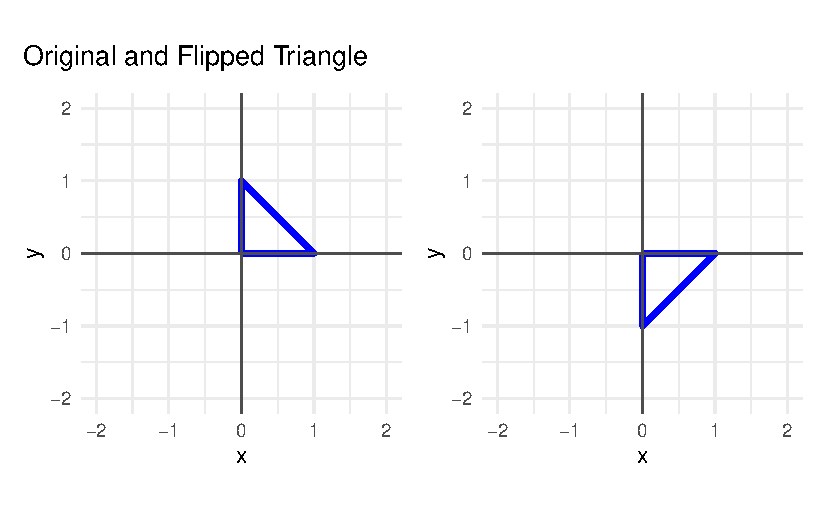
\includegraphics{Assignment-1---Fox_files/figure-pdf/flip-1.pdf}

Finally, we can use transformation matrices to rotate a shape. Below, we
use a transformation matrix rotating our shape 90 degrees clockwise and
repeat four times for a full 360 degrees:

\begin{Shaded}
\begin{Highlighting}[]
\CommentTok{\# create transformation matrix (x, y) → ({-}y, x)}
\NormalTok{matrix\_rotate\_90 }\OtherTok{\textless{}{-}} \FunctionTok{matrix}\NormalTok{(}\FunctionTok{c}\NormalTok{(}\DecValTok{0}\NormalTok{,}\SpecialCharTok{{-}}\DecValTok{1}\NormalTok{,}
                             \DecValTok{1}\NormalTok{, }\DecValTok{0}\NormalTok{),}
                           \AttributeTok{nrow =} \DecValTok{2}\NormalTok{, }\AttributeTok{byrow =} \ConstantTok{TRUE}\NormalTok{)}
\NormalTok{matrix\_rotate\_90}
\end{Highlighting}
\end{Shaded}

\begin{verbatim}
     [,1] [,2]
[1,]    0   -1
[2,]    1    0
\end{verbatim}

\begin{Shaded}
\begin{Highlighting}[]
\CommentTok{\# create list to hold plots for display}
\NormalTok{rotated\_shapes }\OtherTok{\textless{}{-}} \FunctionTok{list}\NormalTok{()}
\NormalTok{rotated\_shapes[[}\DecValTok{1}\NormalTok{]] }\OtherTok{\textless{}{-}}\NormalTok{ plot\_my\_shape}

\NormalTok{current\_shape }\OtherTok{\textless{}{-}} \FunctionTok{t}\NormalTok{(my\_shape)}
\NormalTok{current\_shape}
\end{Highlighting}
\end{Shaded}

\begin{verbatim}
     [,1] [,2]
[1,]    0    0
[2,]    0    1
[3,]    1    0
[4,]    0    0
\end{verbatim}

\begin{Shaded}
\begin{Highlighting}[]
\CommentTok{\# loop: multiply, convert to df, create and store plot}

\ControlFlowTok{for}\NormalTok{ (i }\ControlFlowTok{in} \DecValTok{2}\SpecialCharTok{:}\DecValTok{5}\NormalTok{) \{}
  
  \CommentTok{\# multiply matrix}
\NormalTok{  current\_shape }\OtherTok{\textless{}{-}}\NormalTok{ current\_shape }\SpecialCharTok{\%*\%}\NormalTok{ matrix\_rotate\_90 }
\NormalTok{  current\_shape}
  
  \CommentTok{\# convert transformed matrix to df with column names x,y}
\NormalTok{  df\_rotate\_90 }\OtherTok{\textless{}{-}} \FunctionTok{as.data.frame}\NormalTok{(current\_shape)  }
  \FunctionTok{colnames}\NormalTok{(df\_rotate\_90) }\OtherTok{\textless{}{-}} \FunctionTok{c}\NormalTok{(}\StringTok{"x"}\NormalTok{,}\StringTok{"y"}\NormalTok{)}
  
\NormalTok{  df\_rotate\_90}
  
  \CommentTok{\# create and store plot}
\NormalTok{  rotated\_shapes[[i]] }\OtherTok{\textless{}{-}}\NormalTok{ df\_rotate\_90 }\SpecialCharTok{\%\textgreater{}\%} 
    \FunctionTok{ggplot}\NormalTok{(}\FunctionTok{aes}\NormalTok{(}\AttributeTok{x =}\NormalTok{ x, }\AttributeTok{y =}\NormalTok{ y)) }\SpecialCharTok{+}
    \FunctionTok{geom\_path}\NormalTok{(}\AttributeTok{color =} \StringTok{\textquotesingle{}blue\textquotesingle{}}\NormalTok{, }\AttributeTok{linewidth =} \FloatTok{1.2}\NormalTok{) }\SpecialCharTok{+}
    \FunctionTok{geom\_hline}\NormalTok{(}\AttributeTok{yintercept =} \DecValTok{0}\NormalTok{, }\AttributeTok{color =} \StringTok{"gray30"}\NormalTok{) }\SpecialCharTok{+}
    \FunctionTok{geom\_vline}\NormalTok{(}\AttributeTok{xintercept =} \DecValTok{0}\NormalTok{, }\AttributeTok{color =} \StringTok{"gray30"}\NormalTok{) }\SpecialCharTok{+}
    \FunctionTok{coord\_fixed}\NormalTok{(}\AttributeTok{xlim =} \FunctionTok{c}\NormalTok{(}\SpecialCharTok{{-}}\DecValTok{2}\NormalTok{,}\DecValTok{2}\NormalTok{), }\AttributeTok{ylim =} \FunctionTok{c}\NormalTok{(}\SpecialCharTok{{-}}\DecValTok{2}\NormalTok{,}\DecValTok{2}\NormalTok{)) }\SpecialCharTok{+}
    \FunctionTok{theme\_minimal}\NormalTok{() }
\NormalTok{  \}}

\NormalTok{plot\_display }\OtherTok{\textless{}{-}}\NormalTok{ rotated\_shapes[[}\DecValTok{1}\NormalTok{]] }\SpecialCharTok{+}
\NormalTok{                rotated\_shapes[[}\DecValTok{2}\NormalTok{]] }\SpecialCharTok{+}
\NormalTok{                rotated\_shapes[[}\DecValTok{3}\NormalTok{]] }\SpecialCharTok{+}
\NormalTok{                rotated\_shapes[[}\DecValTok{4}\NormalTok{]] }\SpecialCharTok{+}
\NormalTok{                rotated\_shapes[[}\DecValTok{5}\NormalTok{]]}
\NormalTok{plot\_display }\SpecialCharTok{+} 
  \FunctionTok{plot\_layout}\NormalTok{(}\AttributeTok{ncol =} \DecValTok{5}\NormalTok{) }\SpecialCharTok{+}
  \FunctionTok{plot\_annotation}\NormalTok{(}\StringTok{"Original and Rotated Triangles"}\NormalTok{)}
\end{Highlighting}
\end{Shaded}

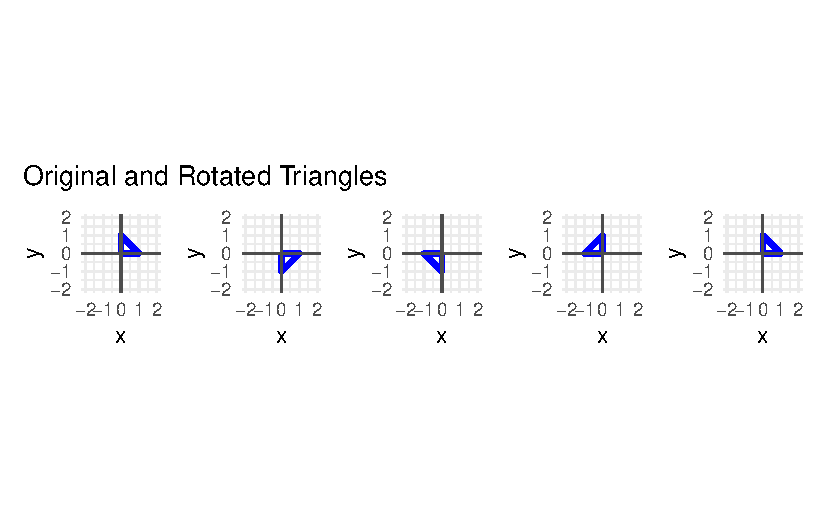
\includegraphics{Assignment-1---Fox_files/figure-pdf/rotate_static-1.pdf}

\subsubsection{2. Proofs \& SVD Example}\label{proofs-svd-example}

\paragraph{\texorpdfstring{A. Prove that
\(A \times B \neq B \times A\)}{A. Prove that A \textbackslash times B \textbackslash neq B \textbackslash times A}}\label{a.-prove-that-a-times-b-neq-b-times-a}

\begin{Shaded}
\begin{Highlighting}[]
\CommentTok{\# {-}{-}{-}{-}{-}{-}{-}{-}{-}{-}{-}{-}{-}{-}}
\CommentTok{\# AB \textless{}\textgreater{} BA}
\CommentTok{\# {-}{-}{-}{-}{-}{-}{-}{-}{-}{-}{-}{-}{-}{-}}

\CommentTok{\# define two 3x3 matrices A and B}

\NormalTok{A }\OtherTok{\textless{}{-}} \FunctionTok{matrix}\NormalTok{(}\FunctionTok{c}\NormalTok{(}\DecValTok{1}\NormalTok{,}\DecValTok{2}\NormalTok{,}\DecValTok{3}\NormalTok{,}
              \DecValTok{4}\NormalTok{,}\DecValTok{5}\NormalTok{,}\DecValTok{6}\NormalTok{,}
              \DecValTok{7}\NormalTok{,}\DecValTok{8}\NormalTok{,}\DecValTok{9}\NormalTok{),}
            \AttributeTok{nrow =} \DecValTok{3}\NormalTok{, }\AttributeTok{byrow =} \ConstantTok{TRUE}\NormalTok{)}

\NormalTok{B }\OtherTok{\textless{}{-}} \FunctionTok{matrix}\NormalTok{(}\FunctionTok{c}\NormalTok{(}\DecValTok{1}\NormalTok{, }\DecValTok{0}\NormalTok{,}\SpecialCharTok{{-}}\DecValTok{1}\NormalTok{,}
              \DecValTok{1}\NormalTok{, }\DecValTok{2}\NormalTok{, }\DecValTok{0}\NormalTok{,}
              \DecValTok{0}\NormalTok{,}\SpecialCharTok{{-}}\DecValTok{1}\NormalTok{, }\DecValTok{1}\NormalTok{),}
            \AttributeTok{nrow =} \DecValTok{3}\NormalTok{, }\AttributeTok{byrow =} \ConstantTok{TRUE}\NormalTok{)}

\NormalTok{A}\SpecialCharTok{\%*\%}\NormalTok{B}
\end{Highlighting}
\end{Shaded}

\begin{verbatim}
     [,1] [,2] [,3]
[1,]    3    1    2
[2,]    9    4    2
[3,]   15    7    2
\end{verbatim}

\begin{Shaded}
\begin{Highlighting}[]
\NormalTok{B}\SpecialCharTok{\%*\%}\NormalTok{A}
\end{Highlighting}
\end{Shaded}

\begin{verbatim}
     [,1] [,2] [,3]
[1,]   -6   -6   -6
[2,]    9   12   15
[3,]    3    3    3
\end{verbatim}

\paragraph{\texorpdfstring{B. Prove that \(A^T*A\) is always
symmetric.}{B. Prove that A\^{}T*A is always symmetric.}}\label{b.-prove-that-ata-is-always-symmetric.}

The matrix \(A^T \times A\) is always symmetric because by transposing
any matrix \(A\) with dimensions \(m \times n\), we get a matrix \(A^T\)
with dimensions \(n \times m\). This has two implications for
multiplying \(A^T \times A\):

\begin{enumerate}
\def\labelenumi{\arabic{enumi}.}
\item
  The multiplication \((n \times m) \times (m \times n)\) always works
  because the number of columns in the first matrix (\(m\)) match the
  number of rows(\(m\)) in the second, which makes matrix multiplication
  possible.
\item
  The resulting matrix has dimensions \(n \times n\), which is square
  and symmetric, because the dimensions are defined by the number of
  rows in the first matrix (\(n\)) and the number of columns in the
  second matrix (also \(n\)).
\end{enumerate}

\begin{Shaded}
\begin{Highlighting}[]
\CommentTok{\# Matrix A from above:}
\NormalTok{A}
\end{Highlighting}
\end{Shaded}

\begin{verbatim}
     [,1] [,2] [,3]
[1,]    1    2    3
[2,]    4    5    6
[3,]    7    8    9
\end{verbatim}

\begin{Shaded}
\begin{Highlighting}[]
\CommentTok{\# Transpose of A:}
\FunctionTok{t}\NormalTok{(A)}
\end{Highlighting}
\end{Shaded}

\begin{verbatim}
     [,1] [,2] [,3]
[1,]    1    4    7
[2,]    2    5    8
[3,]    3    6    9
\end{verbatim}

\begin{Shaded}
\begin{Highlighting}[]
\CommentTok{\# Transpose of A times A:}
\FunctionTok{t}\NormalTok{(A) }\SpecialCharTok{\%*\%}\NormalTok{ A}
\end{Highlighting}
\end{Shaded}

\begin{verbatim}
     [,1] [,2] [,3]
[1,]   66   78   90
[2,]   78   93  108
[3,]   90  108  126
\end{verbatim}

\paragraph{\texorpdfstring{C. Prove that \(det(A^T \times A)\) is
non-negative}{C. Prove that det(A\^{}T \textbackslash times A) is non-negative}}\label{c.-prove-that-detat-times-a-is-non-negative}

\(A^T \times A\) results in a square matrix as shown above, so we can
calculate a determinant.

We also know that \(det(A^T \times A) = det(A)^2\), and also that, like
any square, \(det(A)^2\) must be \(\geq 0\).

Therefore, if \(det(A^T \times A) = det(A)^2\) and \(det(A)^2 \geq 0\)
then \(det(A^T \times A) \geq 0\).

\begin{Shaded}
\begin{Highlighting}[]
\CommentTok{\# determinant of transpose of A times A:}
\FunctionTok{det}\NormalTok{(}\FunctionTok{t}\NormalTok{(A) }\SpecialCharTok{\%*\%}\NormalTok{ A)}
\end{Highlighting}
\end{Shaded}

\begin{verbatim}
[1] -1.534772e-12
\end{verbatim}

\paragraph{D. Singular Value Decomposition (SVD) and Image Compression:
Write an R function that performs Singular Value Decomposition (SVD) on
a grayscale image (which can be represented as a matrix). Use this
decomposition to compress the image by keeping only the top k singular
values and their corresponding vectors. Demonstrate the effect of
different values of k on the compressed image's
quality.}\label{d.-singular-value-decomposition-svd-and-image-compression-write-an-r-function-that-performs-singular-value-decomposition-svd-on-a-grayscale-image-which-can-be-represented-as-a-matrix.-use-this-decomposition-to-compress-the-image-by-keeping-only-the-top-k-singular-values-and-their-corresponding-vectors.-demonstrate-the-effect-of-different-values-of-k-on-the-compressed-images-quality.}

This was a challenging but beneficial exercise demonstrating a practical
application of matrix decomposition. I had never manipulated images
before so R function help and online resources (ChatGPT for coding
assistance; see Works Cited) were particularly helpful in
problem-solving this exercise as I worked my way through understanding
the data behind images and manipulating that data in R as matrices.

First, I used a black and white image that turned out to be encoded as
RGB. I learned this is common for compatibility reasons, but all
channels will have the same values for a grayscale image: this meant I
could extract any channel in order to apply SVD with a simple R
function.

Then I extracted the components U, S, and V and created a function to
reconstruct the image matrices for various values of k (ChatGPT). The
first iteration resulted in appropriately compressed images but in
shades of red and rotated -90 degrees. Changing to gray was easy but I
found multiple explanations for rotating the images; a matrix approach
was most helpful to my understanding in the context of this assignment.
While I could not multiply by a transformation matrix directly, the
earlier rotation exercise was helpful in understanding how to manipulate
the x,y points as rows/columns in an image, while the image matrix
expressed the intensity.

The resulting transformed images were compressed relative to the k
value: low values for k (5, 40) showed significant loss of detail, while
a higher value (80) was much closer to the original image, but still not
as sharp.

\begin{Shaded}
\begin{Highlighting}[]
\CommentTok{\# import image and convert to matrix}

\NormalTok{my\_url }\OtherTok{\textless{}{-}} \StringTok{"https://raw.githubusercontent.com/AmandaSFox/DATA605/main/OC1Y7T0.jpg"}
\NormalTok{my\_image }\OtherTok{\textless{}{-}} \FunctionTok{readJPEG}\NormalTok{(}\FunctionTok{getURLContent}\NormalTok{(my\_url, }\AttributeTok{binary =} \ConstantTok{TRUE}\NormalTok{))}

\CommentTok{\# check if three channels (RGB) and if so, extract one channel to make it grayscale}
\ControlFlowTok{if}\NormalTok{(}\FunctionTok{length}\NormalTok{(}\FunctionTok{dim}\NormalTok{(my\_image)) }\SpecialCharTok{==} \DecValTok{3}\NormalTok{) \{}
\NormalTok{  my\_image }\OtherTok{\textless{}{-}}\NormalTok{ my\_image[, , }\DecValTok{1}\NormalTok{] }
\NormalTok{  \}}

\CommentTok{\# validate image size and not three dimensions }
\FunctionTok{dim}\NormalTok{(my\_image)}
\end{Highlighting}
\end{Shaded}

\begin{verbatim}
[1] 1300 1300
\end{verbatim}

\begin{Shaded}
\begin{Highlighting}[]
\CommentTok{\# apply SVD and display components}
\NormalTok{my\_svd }\OtherTok{\textless{}{-}} \FunctionTok{svd}\NormalTok{(my\_image)}

\CommentTok{\# Extract components}
\NormalTok{U }\OtherTok{\textless{}{-}}\NormalTok{ my\_svd}\SpecialCharTok{$}\NormalTok{u}
\NormalTok{S }\OtherTok{\textless{}{-}} \FunctionTok{diag}\NormalTok{(my\_svd}\SpecialCharTok{$}\NormalTok{d) }
\NormalTok{V }\OtherTok{\textless{}{-}}\NormalTok{ my\_svd}\SpecialCharTok{$}\NormalTok{v}

\CommentTok{\# Reconstruct image FUNCTION}
\NormalTok{reconstruct\_image }\OtherTok{\textless{}{-}} \ControlFlowTok{function}\NormalTok{(k) \{}
\NormalTok{  U\_k }\OtherTok{\textless{}{-}}\NormalTok{ U[, }\DecValTok{1}\SpecialCharTok{:}\NormalTok{k]  }\CommentTok{\# First k columns of U}
\NormalTok{  S\_k }\OtherTok{\textless{}{-}}\NormalTok{ S[}\DecValTok{1}\SpecialCharTok{:}\NormalTok{k, }\DecValTok{1}\SpecialCharTok{:}\NormalTok{k]  }\CommentTok{\# Top k singular values}
\NormalTok{  V\_k }\OtherTok{\textless{}{-}}\NormalTok{ V[, }\DecValTok{1}\SpecialCharTok{:}\NormalTok{k]  }\CommentTok{\# First k columns of V}
\NormalTok{  img\_k }\OtherTok{\textless{}{-}}\NormalTok{ U\_k }\SpecialCharTok{\%*\%}\NormalTok{ S\_k }\SpecialCharTok{\%*\%} \FunctionTok{t}\NormalTok{(V\_k)}
  \FunctionTok{return}\NormalTok{(img\_k)}
\NormalTok{\}}

\CommentTok{\# Substitute different k values and create three new matrices: }
\NormalTok{img\_k5 }\OtherTok{\textless{}{-}} \FunctionTok{reconstruct\_image}\NormalTok{(}\DecValTok{5}\NormalTok{)}
\NormalTok{img\_k40 }\OtherTok{\textless{}{-}} \FunctionTok{reconstruct\_image}\NormalTok{(}\DecValTok{30}\NormalTok{)}
\NormalTok{img\_k80 }\OtherTok{\textless{}{-}} \FunctionTok{reconstruct\_image}\NormalTok{(}\DecValTok{80}\NormalTok{)}

\CommentTok{\# create function to correct rotation:      }
\NormalTok{rotate\_90 }\OtherTok{\textless{}{-}} \ControlFlowTok{function}\NormalTok{(image\_matrix) \{}
\NormalTok{  rotated\_matrix }\OtherTok{\textless{}{-}} \FunctionTok{t}\NormalTok{(image\_matrix)[, }\FunctionTok{ncol}\NormalTok{(image\_matrix)}\SpecialCharTok{:}\DecValTok{1}\NormalTok{]}
  \FunctionTok{return}\NormalTok{(rotated\_matrix)}
\NormalTok{\}}

\CommentTok{\# setting to display all images in one row}
\FunctionTok{par}\NormalTok{(}\AttributeTok{mfrow =} \FunctionTok{c}\NormalTok{(}\DecValTok{1}\NormalTok{,}\DecValTok{4}\NormalTok{))}

\CommentTok{\# create four images, applying above rotation function, gray instead of red}
\NormalTok{my\_image\_k5 }\OtherTok{\textless{}{-}} \FunctionTok{image}\NormalTok{(}\FunctionTok{rotate\_90}\NormalTok{(img\_k5), }\AttributeTok{col =} \FunctionTok{gray.colors}\NormalTok{(}\DecValTok{256}\NormalTok{), }\AttributeTok{main=}\StringTok{"k = 5"}\NormalTok{)}
\NormalTok{my\_image\_k40 }\OtherTok{\textless{}{-}} \FunctionTok{image}\NormalTok{(}\FunctionTok{rotate\_90}\NormalTok{(img\_k40), }\AttributeTok{col =} \FunctionTok{gray.colors}\NormalTok{(}\DecValTok{256}\NormalTok{), }\AttributeTok{main=}\StringTok{"k = 40"}\NormalTok{)}
\NormalTok{my\_image\_k80 }\OtherTok{\textless{}{-}} \FunctionTok{image}\NormalTok{(}\FunctionTok{rotate\_90}\NormalTok{(img\_k80), }\AttributeTok{col =} \FunctionTok{gray.colors}\NormalTok{(}\DecValTok{256}\NormalTok{), }\AttributeTok{main=}\StringTok{"k = 80"}\NormalTok{)}
\NormalTok{my\_image\_orig }\OtherTok{\textless{}{-}} \FunctionTok{image}\NormalTok{(}\FunctionTok{rotate\_90}\NormalTok{(my\_image), }\AttributeTok{col =} \FunctionTok{gray.colors}\NormalTok{(}\DecValTok{256}\NormalTok{), }\AttributeTok{main=}\StringTok{"Original"}\NormalTok{)}
\end{Highlighting}
\end{Shaded}

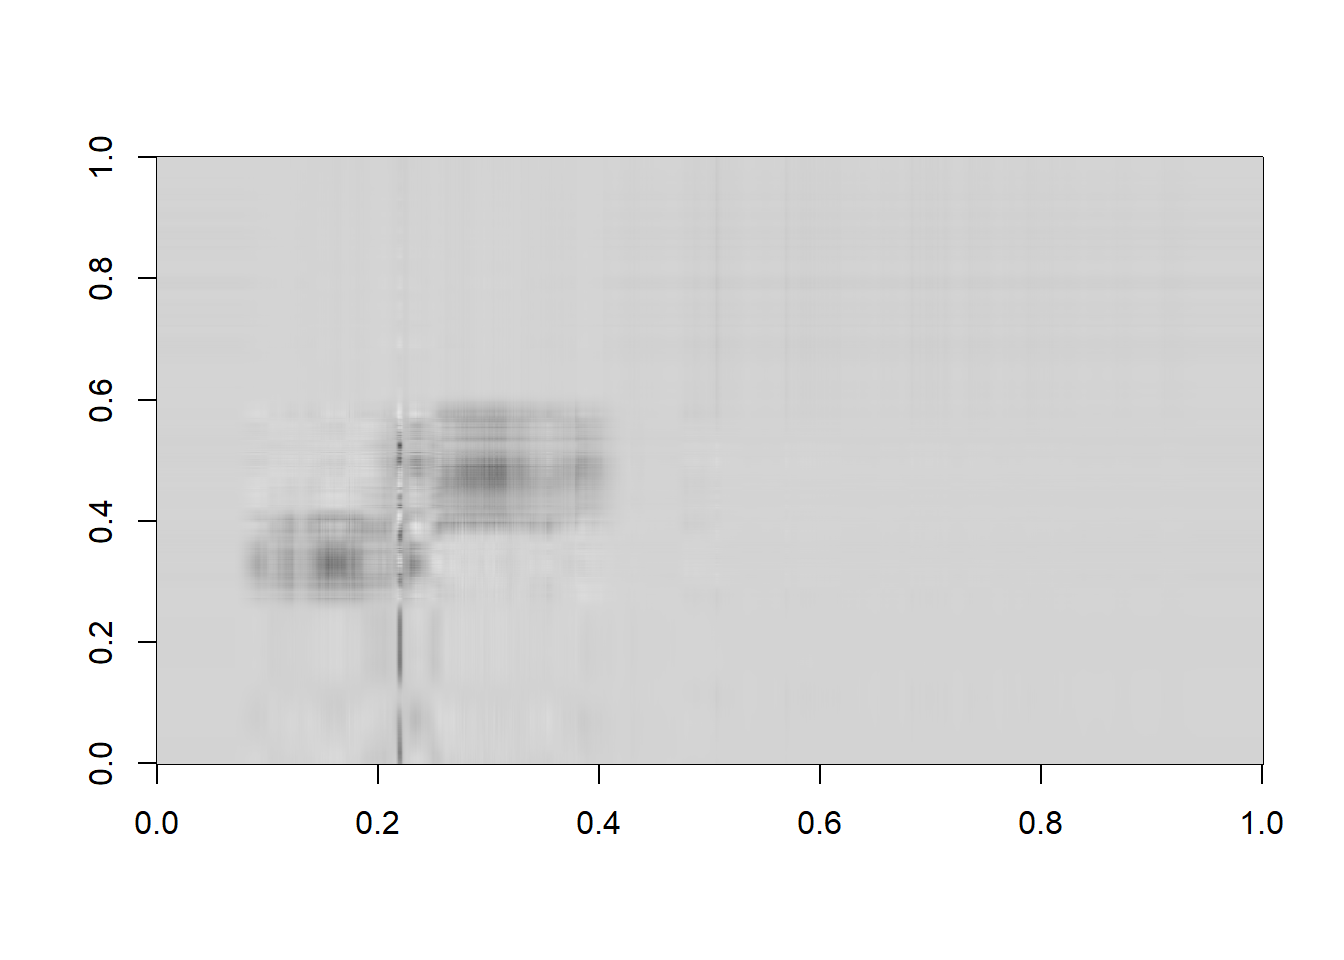
\includegraphics{Assignment-1---Fox_files/figure-pdf/import_image-1.pdf}



\end{document}
